\section{Rapport \textit{Effectors} Implementation}
\label{sec:rapportStrategies}

The following section describes the most relevant implementation details of the rapport \textit{Effectors} of the model detailed in Chapter~\ref{chap:rapportModel}. As denoted in Sections~\ref{sub:model_positivity}, \ref{sub:model_Coordination}, and \ref{sec:mutual_attentionModel}, the rapport strategies have to be parametrisable, so that researchers may adapt the model to any agent embodiment or \ac{HRI} scenario. 

The Positivity rapport \textit{Effector} (that satisfies the ``Stimulate positivity'' goal) and the ``Adhere to Social Norms'' goal are implemented by triggering utterances given the perceptual information of the scenario. Finally, The \textit{Effectors} were implemented and tested using robot \ac{EMYS} (Figure~\ref{fig:robots:EMYS2}).


%TODO referir que a positivity e o adhere to social norms são implementados scenario based

%In the following sections we will describe the supporting technologies, \ac{SSI}~\cite{Wagner2013}, SHORE~\cite{Ruf2011}, and GRETA~\cite{Niewiadomski2009} in Section~\ref{sec:supportingTechnologies}, followed by a brief description of the \textit{Effectors} described above.

%Most of all, in order to build rapport more effectively, one should take into consideration if the above-mentioned strategies fit the study scenario, and if they are adequate to the person the agent is interacting with (e.g., introvert and extrovert people should be handled differently~\cite{Andrist2015}). This aspect is more relevant for enhancing positivity which is mostly built either through vocal interactions or through gestures. For this purpose, in order to build positivity, the developer must build their own \textit{Effector} or \textit{Effectors}.



% Bull1981, Baxter2014
% Impact on users behaviour
%Buschmeier2011, Zhao2014, Reidsma2011, Gratch2006, Mutlu2006, Andrist2015, Stanton2014,


\subsection{Supporting Technologies}
\label{sec:supportingTechnologies}

Revisiting the rapport model described throughout Chapter~\ref{chap:rapportModel}, the rapport \textit{Effectors} require the following perceptual capabilities:
\begin{itemize}
	\item Monitor the interaction activity, for the Positivity \textit{Effectors}.
	\item Identify human emotions, and head-gestures for the behavioural mimicry \textit{Effectors};
	\item Identify speech disfluencies (Figures~\ref{fig:lowering} to \ref{fig:risingLowering}) for the backchannel \textit{Effector};
	\item Identify the user's gender and monitor the current state of the interaction, for the Mutual-Gaze \textit{Effector};
\end{itemize}

Following Figure~\ref{fig:SupportingTechnologiesOverview}, the system uses \ac{SSI}~\footnote{\url{http://hcm-lab.de/projects/ssi/}} to recognise social-signals in real-time from microphones and video feeds~\cite{Wagner2013}. \ac{SSI} uses SHORE~\cite{Ruf2011} and openSMILE~\cite{Eyben:2013:RDO:2502081.2502224} to recognise emotions, and extract prosody features, respectively. For example, \ac{SSI} identifies head-gestures using a Kinect Camera, and SHORE outputs the different emotion intensities given the video feed. Finally, \ac{SSI} periodically collects and sends the perceptual information in \ac{XML} format through network messages to other processes using ActiveMQ~\footnote{\url{http://activemq.apache.org/}}, specifically GRETA\textsuperscript{PP}.

\begin{figure}[H]
	\centering
	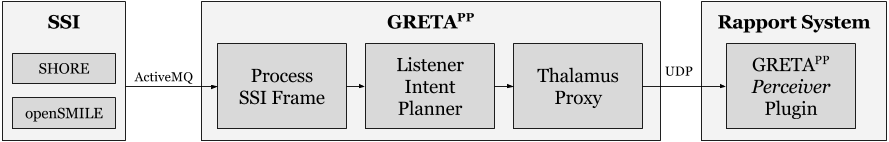
\includegraphics[width=0.95\textwidth]{images/SupportingTechnologiesOverview.png}
	\caption{Schematic representation of the components that supports the rapport model.}
	\label{fig:SupportingTechnologiesOverview}
\end{figure}

GRETA\textsuperscript{PP} is a variation of the GRETA system~\cite{Niewiadomski2009} that uses only the  \textit{Listener Intention Planner} component of the original GRETA (Figure~\ref{fig:GretaOriginal}), as we are not interested in the remaining components for the scope of this thesis. In short, GRETA\textsuperscript{PP} attempts to match the perceptual information to the first behavioural rule defined in a configuration file loaded at launch as exampled in Listing~\ref{lst:exampleGretaRule}. In the case of a match, the system might output a response signal given the response probability specified by the same rule. The original set of rules was reduced, as they were tailored for a virtual agent with different capabilities than the robot \ac{EMYS}, for example, the virtual agent is capable of moving his eyebrows and specific lip positions. Finally, taking advantage that GRETA is already integrated with \ac{SSI}, we adapted \ac{SSI} and GRETA\textsuperscript{PP} to redirect head gestures and facial expressions perceptual information to our system. It is important to mention that there is a slight delay beginning from \ac{SSI} and ending in the \textit{Perceiver}, and that only the emotion with the highest intensity is sent. The major bottleneck of the system relies on \ac{SSI} itself which is resource intensive and, in order to be able to test the system, the refresh rate had to be reduced to 5Hz which is half the default value.


\begin{lstlisting}[caption={One of the backchannels rules used GRETA and GRETA\textsuperscript{PP}.},label={lst:exampleGretaRule},language=XML]
<rule name="trigger-rise-fall">
	<usersignals>
		<usersignal id="1" name="rise_fall" modality="speech"/>
	</usersignals>
	<backchannels probability="1.0" priority="2">
		<response_reactive probability="0.4"/>
	</backchannels>
</rule>
\end{lstlisting}

Lastly, the communication with the rapport system is accomplished using \ac{UDP} sockets to transmit information in real-time without concerning with packet-loss as the system runs locally. The GRETA\textsuperscript{PP} \textit{Perceiver} Plugin, given the perceptual information, will notify the interested \textit{Effectors}.

\begin{figure}[H]
	\centering
	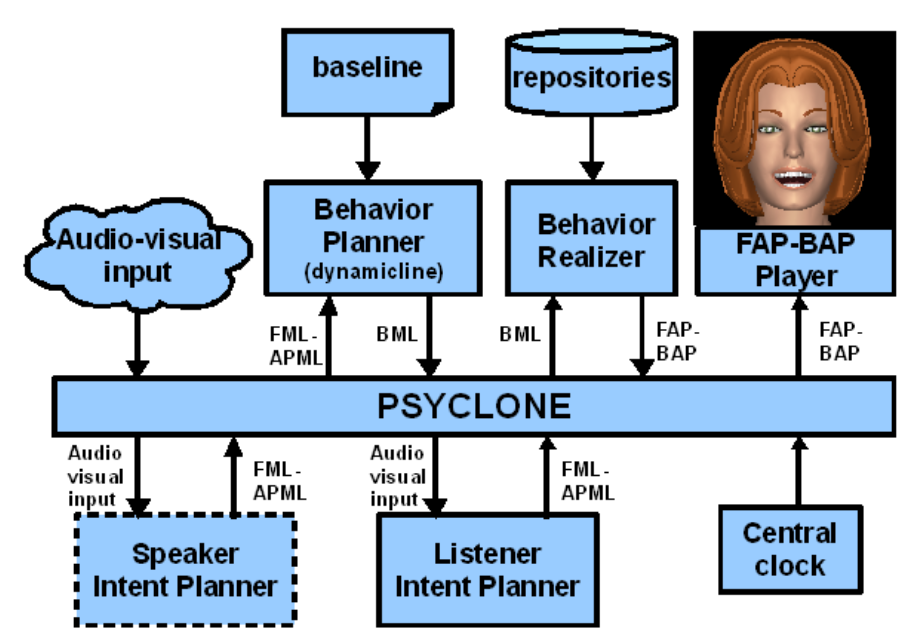
\includegraphics[width=0.6\textwidth]{images/GretaArchitecture.png}
	\caption{GRETA architecture. From~\cite{Niewiadomski2009}}
	\label{fig:GretaOriginal}
\end{figure}



% there are four main modules  that supports the rapport strategies:
%\begin{itemize}
%	\item \textbf{\ac{SSI}}: recognise social signals in realtime;
%	\item \textbf{SHORE}: recognise emotions from a video feed;
%	\item \textbf{GRETA\textsuperscript{PP}}: adapted version of GRETA~\cite{Niewiadomski2009} to generate listener behaviour;
%	\item \textbf{GRETA \textit{Perceiver} Plugin}: proxy between GRETA\textsuperscript{PP} and the \textit{Rapport Controller}.
%\end{itemize}


\subsection{Facial Expression Mimicry}
\label{sub:sec:FacialExpressionMimicry}

The Facial Expression Mimicry rapport \textit{Effector} mimics the user's emotion given the perceptual information returned from SHORE (the source code is available in listing~\ref{lst:facialExpressionsSourceCode} in Appendix C). The \textit{Effector}'s parameters (Table~\ref{table:facialMimicryParameters}) were attributed empirically following several pilots that were run with 3 different people until a balance was found between overeagerness and lack of liveness (Table~\ref{table:facialMimicryParametersValues}). In particular, the probability and the minimum delay specified in Table~\ref{table:facialMimicryParametersValues} were crucial to avoid triggering animations one, after another, for the duration of the emotion. In addition, the final \textit{Nutty Tracks} animation identifier is the base identifier followed by a random number between 1 and 5, for example, \textit{sadness1}, \textit{joy4}, and \textit{surprise3}. With this randomisation, the agent will not be as repetitive which may impact negatively the user's opinion of it. %Lastly, Anger is not specified as SHORE often mistakes it for happiness.

Nonetheless, the implementation of this plugin is not without issues as:
\begin{itemize}
    \item In absence of faces, SHORE outputs happiness emotions with a high level of intensity ($>$ 75);
    \item There is a slight noticeable delay (less than 1 second) between the emotion appearing on the video feed and being transmitted to GRETA;
    \item Camera distance and light conditions have the greatest impact on accuracy.
\end{itemize}

The issues lied on a balance between accuracy and speed. Applying a smoothing filter solved the second issue by reducing the signal spikes but it increased the delay from at most 1 second to 3 seconds. In the end, we opted to remove the smoothing filter, compensating with enabling/disabling this plugin only when required in runtime (Section~\ref{sub:sec:effectorPlugin}). Finally, the last issue is easily solved by taking the lightning conditions into consideration when preparing the physical space.

\begin{table}[H]
	\centering
	\begin{tabular}{|l|c|c|c|}
	\hline
	\multicolumn{1}{|c|}{\textbf{Parameter}} & \textbf{Happiness} & \textbf{Sadness} & \textbf{Surprise} \\ \hline
		Priority & 1 & 1 & 1 \\ \hline
		Minimum Intensity & 0.65 & 0.65 & 0.5 \\ \hline
		Trigger Probability & 0.48 & 0.48 & 0.48 \\ \thickhline
		\textit{Nutty Tracks} Base Animation & joy & sadness & surprise \\ \hline
		Minimum delay between mimicry behaviours (ms) & 3500 & 3500 & 3500 \\ \hline	
	\end{tabular}
	\caption{Parametrisation of the Facial Expression Mimicry rapport \textit{Effector}. }
	\label{table:facialMimicryParametersValues}
\end{table}


\subsection{Head Gesture Mimicry}
\label{sub:sec:HeadNodMimicry}

The Head Gesture Mimicry rapport \textit{Effector} mimics up-down nod gestures and left-right head shakes given the perceptual information returned from \ac{SSI}. In order to make \ac{EMYS} mimic head gestures, we added head nods and head shakes animations to \textit{Nutty Tracks} that takes into account the \textit{Effector} parameters specified in Table~\ref{table:headNodMimicryParameters}. The \textit{Effector} parameters were attributed empirically similar to Facial Expression Mimicry \textit{Effector} (Table~\ref{table:headGesturesMimicryParametersValues}), however, as the sensors seldom detected head gestures during the pilot tests, both gestures' probabilities were set to 1, that is, the agent will always mimic the behaviour.

Lastly, similarly to Facial Expression Mimicry \textit{Effector}, there is an apparent latency between the user's action and the mimicry behaviour, that is only solved by increasing the computational resources.

\begin{table}[H]
	\centering
	\begin{tabular}{|l|c|c|}
	\hline
	\multicolumn{1}{|c|}{\textbf{Parameter}} & \textbf{Up-Down Nods} & \textbf{Left-Right Shakes} \\ \hline
		Priority & 1 & 1 \\ \hline
		Trigger Probability & 1 & 1 \\ \hline
		Intensity Range ($I_{min}$, $I_{max}$) & (10,20) & (40,60) \\ \hline
		Repetitions Range ($R_{min}$, $R_{max}$) & (2,2) & (2,2)\\ \hline
		Frequency Range ($F_{min}$, $F_{max}$) &  (40,55) & (40,55)\\ \thickhline		
		Minimum delay between mimicry behaviours (ms) & 3500 & 3500 \\ \hline		
	\end{tabular}
	\caption{Parametrisation of the Head Gesture Mimicry rapport \textit{Effector}.}
	\label{table:headGesturesMimicryParametersValues}
\end{table}
\subsection{Mutual Gaze}
\label{sub:sec:GazeFace}

The Mutual-Gaze rapport \textit{Effector}, as described in Section~\ref{sec:mutual_attentionModel}, swaps the gaze target depending on the user's personality and on the current state of the interaction, more precisely, whenever the agent is in an in-task phase, or in a between-task phase. As we not know the personality of the user beforehand, the \textit{Effector} assumes that the interactional partner is extroverted (which has lower standard deviation than introvert following Table~\ref{table:gazetimes}). This \textit{Effector} plugin uses the rapport model's default durations parameters which are represented in Table~\ref{table:mutualGazeParametersValues}. Finally, the gaze targets identifiers depicted on the same table are known by \textit{Skene} who triggers the appropriate animations on \textit{Nutty Tracks}.

\begin{table}[H]
	\centering
	\begin{tabular}{|l|c|c|}
	\hline
	\multicolumn{2}{|c|}{\textbf{Parameter}} & \textbf{Value} \\ \hline
	\multicolumn{2}{|l|}{In-task Gaze Priority} & 1 \\ \hline
	\multicolumn{2}{|l|}{Between-tasks Gaze Priority} & 1 \\ \hline
	\multirow{2}{*}{In-task} & Face & 2660 \\ \cline{2-3} 
	 & Task & 4040 \\ \hline
	\multirow{2}{*}{Between-tasks} & Face & 3910 \\ \cline{2-3} 
	 & Task & 1010 \\ \thickhline
	\multicolumn{2}{|l|}{Face Gaze Target Identifier} & middleFront \\ \hline
	\multicolumn{2}{|l|}{Task Gaze Target Identifier} & bottomFront \\ \hline
	\end{tabular}
	\caption{Parametrisation of the Mutual Gaze rapport \textit{Effector}.}
	\label{table:mutualGazeParametersValues}
\end{table}

%Despite SHORE being capable of estimating accurately the gender of the user, it must be defined beforehand by the developer. 








%table:mutualGazeParameters
%table:backchannel
%table:headNodMimicryParameters


\subsection{Backchannel}
\label{sub:sec:backchannel}

The Backchannel rapport \textit{Effector} is based on the work developed on the GRETA system~\cite{Niewiadomski2009}, that analyses the variations of the pitch perceived by the openSMILE component of \ac{SSI}. Given the backchannel timings received from the GRETA\textsuperscript{PP} \textit{Perceiver} plugin, the \textit{Effector} plugin produces only head nods, as we were not able to generate a convincing \textit{Hmm hmmm} with a similar pitch as the generated voice by the \textit{Speech Server}. Ideally, the agent would alternate between head nods, \textit{Hmm hmmm} vocalisations, or both head nods and vocalisations. The parameters' values are depicted in Table~\ref{table:headGesturesMimicryParametersValues}, which are almost identical to the ones used in the Head Gesture Mimicry \textit{Effector}, except the priority is higher as the action proposals are executed on discrete states of the interaction. The trigger probability is identical to the one used in GRETA.

Despite succeeding with the integration of \ac{SSI} and GRETA, the resulting Backchannel \textit{Effector} did not behave as expected due to environmental factors that could not be controlled without changing the agent's embodiment as:
\begin{itemize}
	\item The \ac{EMYS}'s movement are noisy;
	\item The \ac{EMYS}'s voice is played through external speakers.
\end{itemize}

We attempted to reduce the impact of these factors by:
\begin{itemize}
	\item Use directional noise-suppressing microphone;
	\item Reduce the microphone sensivity;
	\item Adapt the \ac{SSI} pipeline to increase the pitch baseline.
\end{itemize}

To conclude, despite these efforts, this \textit{Effector} did not behave as intended, therefore it was not used in the user studies in Chapter~\ref{chap:userstudies}.

\begin{table}[H]
	\centering
	\begin{tabular}{|l|c|}
	\hline
	\multicolumn{1}{|c|}{\textbf{Parameter}} & \textbf{Backchannel Head Nod}\\ \hline
		Priority & 2 \\ \hline
		Trigger Probability & 0.4 \\ \hline
		Intensity Range ($I_{min}$, $I_{max}$) & (10,20) \\ \hline
		Repetitions Range ($R_{min}$, $R_{max}$) & (2,2) \\ \hline
		Frequency Range ($F_{min}$, $F_{max}$) &  (40,55) \\ \thickhline		
		Minimum delay between mimicry behaviours (ms) & 5000 \\ \hline		
	\end{tabular}
	\caption{Parametrisation of the Backchannel rapport \textit{Effector}.}
	\label{table:headGesturesMimicryParametersValues}
\end{table}

\section{Final Remarks}
During the previous sections, the document describes the system that implements the rapport model described in Chapter~\ref{chap:rapportModel} and extends the \ac{SERA} ecosystem to create robotic agents capable of managing rapport following current literature on models that tailor behavioural strategies to the dyadic state of the interaction. The presented \textit{Effectors} were developed and tested for robot \ac{EMYS} (Figure~\ref{fig:robots:EMYS2}), therefore the values described in Tables~\ref{table:facialMimicryParametersValues} to~\ref{table:headGesturesMimicryParametersValues} are tailored to this embodiment. Auxiliary plugins may have been developed by the researcher to monitor the scenario and trigger contextual utterances that will attempt to enhance positivity and build rapport.  In additional, the system aids the development of customisable plugins so that they can be easily changed by non-technical researchers such as psychiatrists whose knowledge on \ac{HRI} is crucial to building agents. Finally, and above all, pilot tests should be done so that the final set of possible actions sent by the agent are effective on satisfying the interactional goals of the scenario and manage rapport with the user.


%, and on the work developed by Huang et. al.~\ref{Buschmeier2011} on a virtual rapport agent. 
%Limited backchannel behaviours 


